%% This is an example first chapter.  You should put chapter/appendix that you
%% write into a separate file, and add a line \include{yourfilename} to
%% main.tex, where `yourfilename.tex' is the name of the chapter/appendix file.
%% You can process specific files by typing their names in at the 
%% \files=
%% prompt when you run the file main.tex through LaTeX.
\chapter{Application of DEnHKF to Hydrologic Model}

\section{daWUAPhydroengine}

The \textbf{daWUAPhydroengine} hydrologic dynamic model is used to test the viability of the DEnHKF method.  \textbf{daWUAPhydroengine} takes streamflow and subbasin parameters, precipitation, minimum temperatures, and maximum temperatures as inputs and outputs streamflow data along with some additional states such as snow water equivalent. \textbf{daWUAPhydroengine} was designed to be implemented in any geographic location. For this study it was utilized to model streamflows throughout the state of Montana.

\begin{table}[]
\caption{States} 
\begin{tabular}{lll}
State ($x$) & Purpose                              & Dimensions  \\ \hline
streamflow  & Streamflow (in cumecs)               & 330   \\
swe         & Snow Water Equivalent  (in $mm^{3}$) & 45012
\end{tabular}
\label{tab:states}
\end{table}

Configuring \textbf{daWUAPhydroengine} to model streamflows throughout Montana is advantageous because it allows for the calibration of a very large number of spatially distributed, high dimensional parameters. These parameters span the entirety of Montana, which covers an area of 380,800 $km^{2}$. Montana's large geographical coverage is diverse and the terrain differs in various ways (soil composition, forestation, etc.)

\begin{table}[]
\caption{Forcing Data} 
\begin{tabular}{lll}
Forcing Data ($u$) & Purpose                          & Dimensions \\ \hline
tempmin          & Lowest temperature for timestep  & 45012 \\
tempmax          & Highest temperature for timestep & 45012 \\
precipitation      & Amount of rainfall for timestep & 45012 
\end{tabular}
\label{tab:u_params}
\end{table}

\begin{table}[]
\caption{Calibrated Parameters} 
\begin{tabular}{lll}
Parameter ($\theta$) & Purpose                                                    & Dimensions  \\ \hline
ddf                  & Controls Rate of Snowfall                                        & 45012 \\
aet\_lp              & Controls AET                                                      & 45012 \\
soil\_beta           & Controls portion of ponded water that goes into soil storage & 45012 \\
soil\_max\_wat       & Controls soil maximum water capacity & 45012
\end{tabular}
\label{tab:t_params}
\end{table}

\begin{figure}[h]
    \centering
    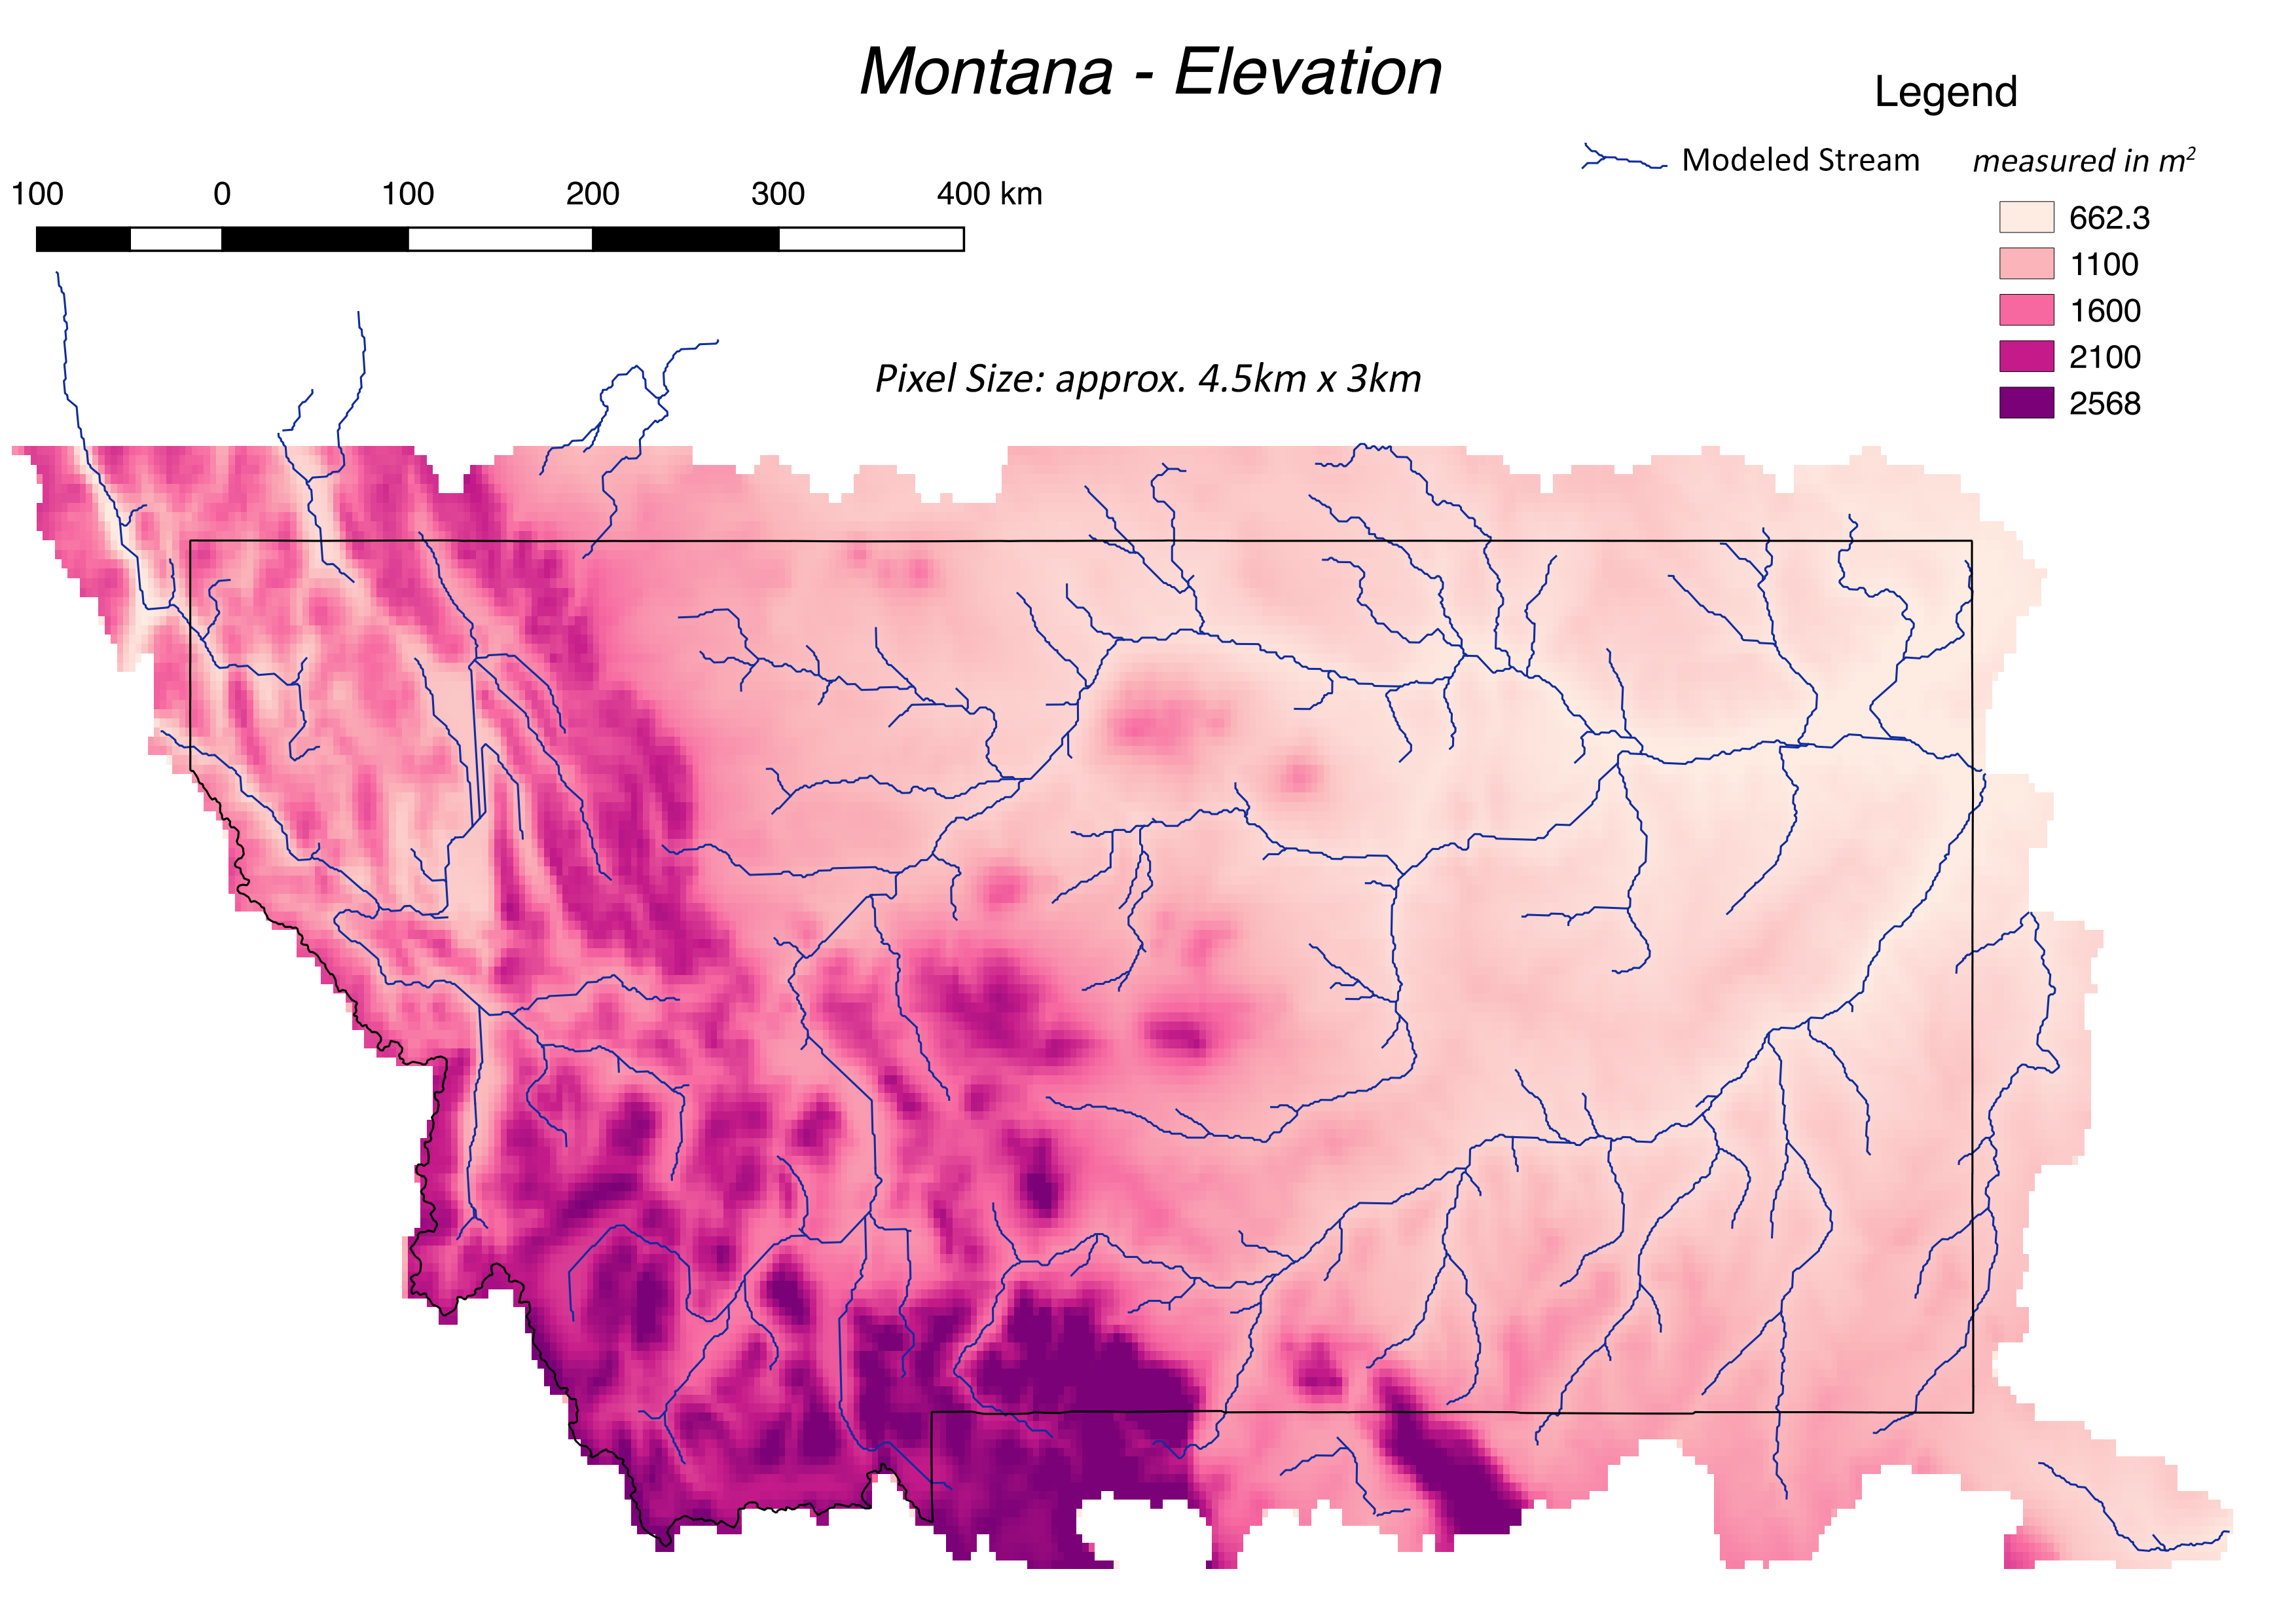
\includegraphics[width=0.95\textwidth]{elevation}
    \caption{Elevation throughout Montana}
    \label{fig:elevation}
\end{figure}

\section{Observation Data}

A Kalman Filter relies on one or more observed states for correction. Accordingly, observations were obtained for streamflows across Montana and snowfall across Montana. For streamflow, USGS streamflow data was collected at 86 sites. Each observed site was paired with the closest simulated \textbf{daWUAPhydroengine} stream outlet within a 2.5 mile cutoff. For snowfall, SNOWTEL sites monitored by the Natural Resources Conservation Service (NRCS) were used. 90 stations were chosen and matched to specific pixels in \textbf{daWUAPhydroengine}'s raster files.


\begin{table}[]
\caption{Observations} 
\begin{tabular}{lll}
Observed State ($x$) & Source                              & Dimensions  \\ \hline
streamflow  & USGS & 82   \\
swe         & NRCS & 90
\end{tabular}
\label{tab:obs}
\end{table}

\begin{figure}[h]
    \centering
    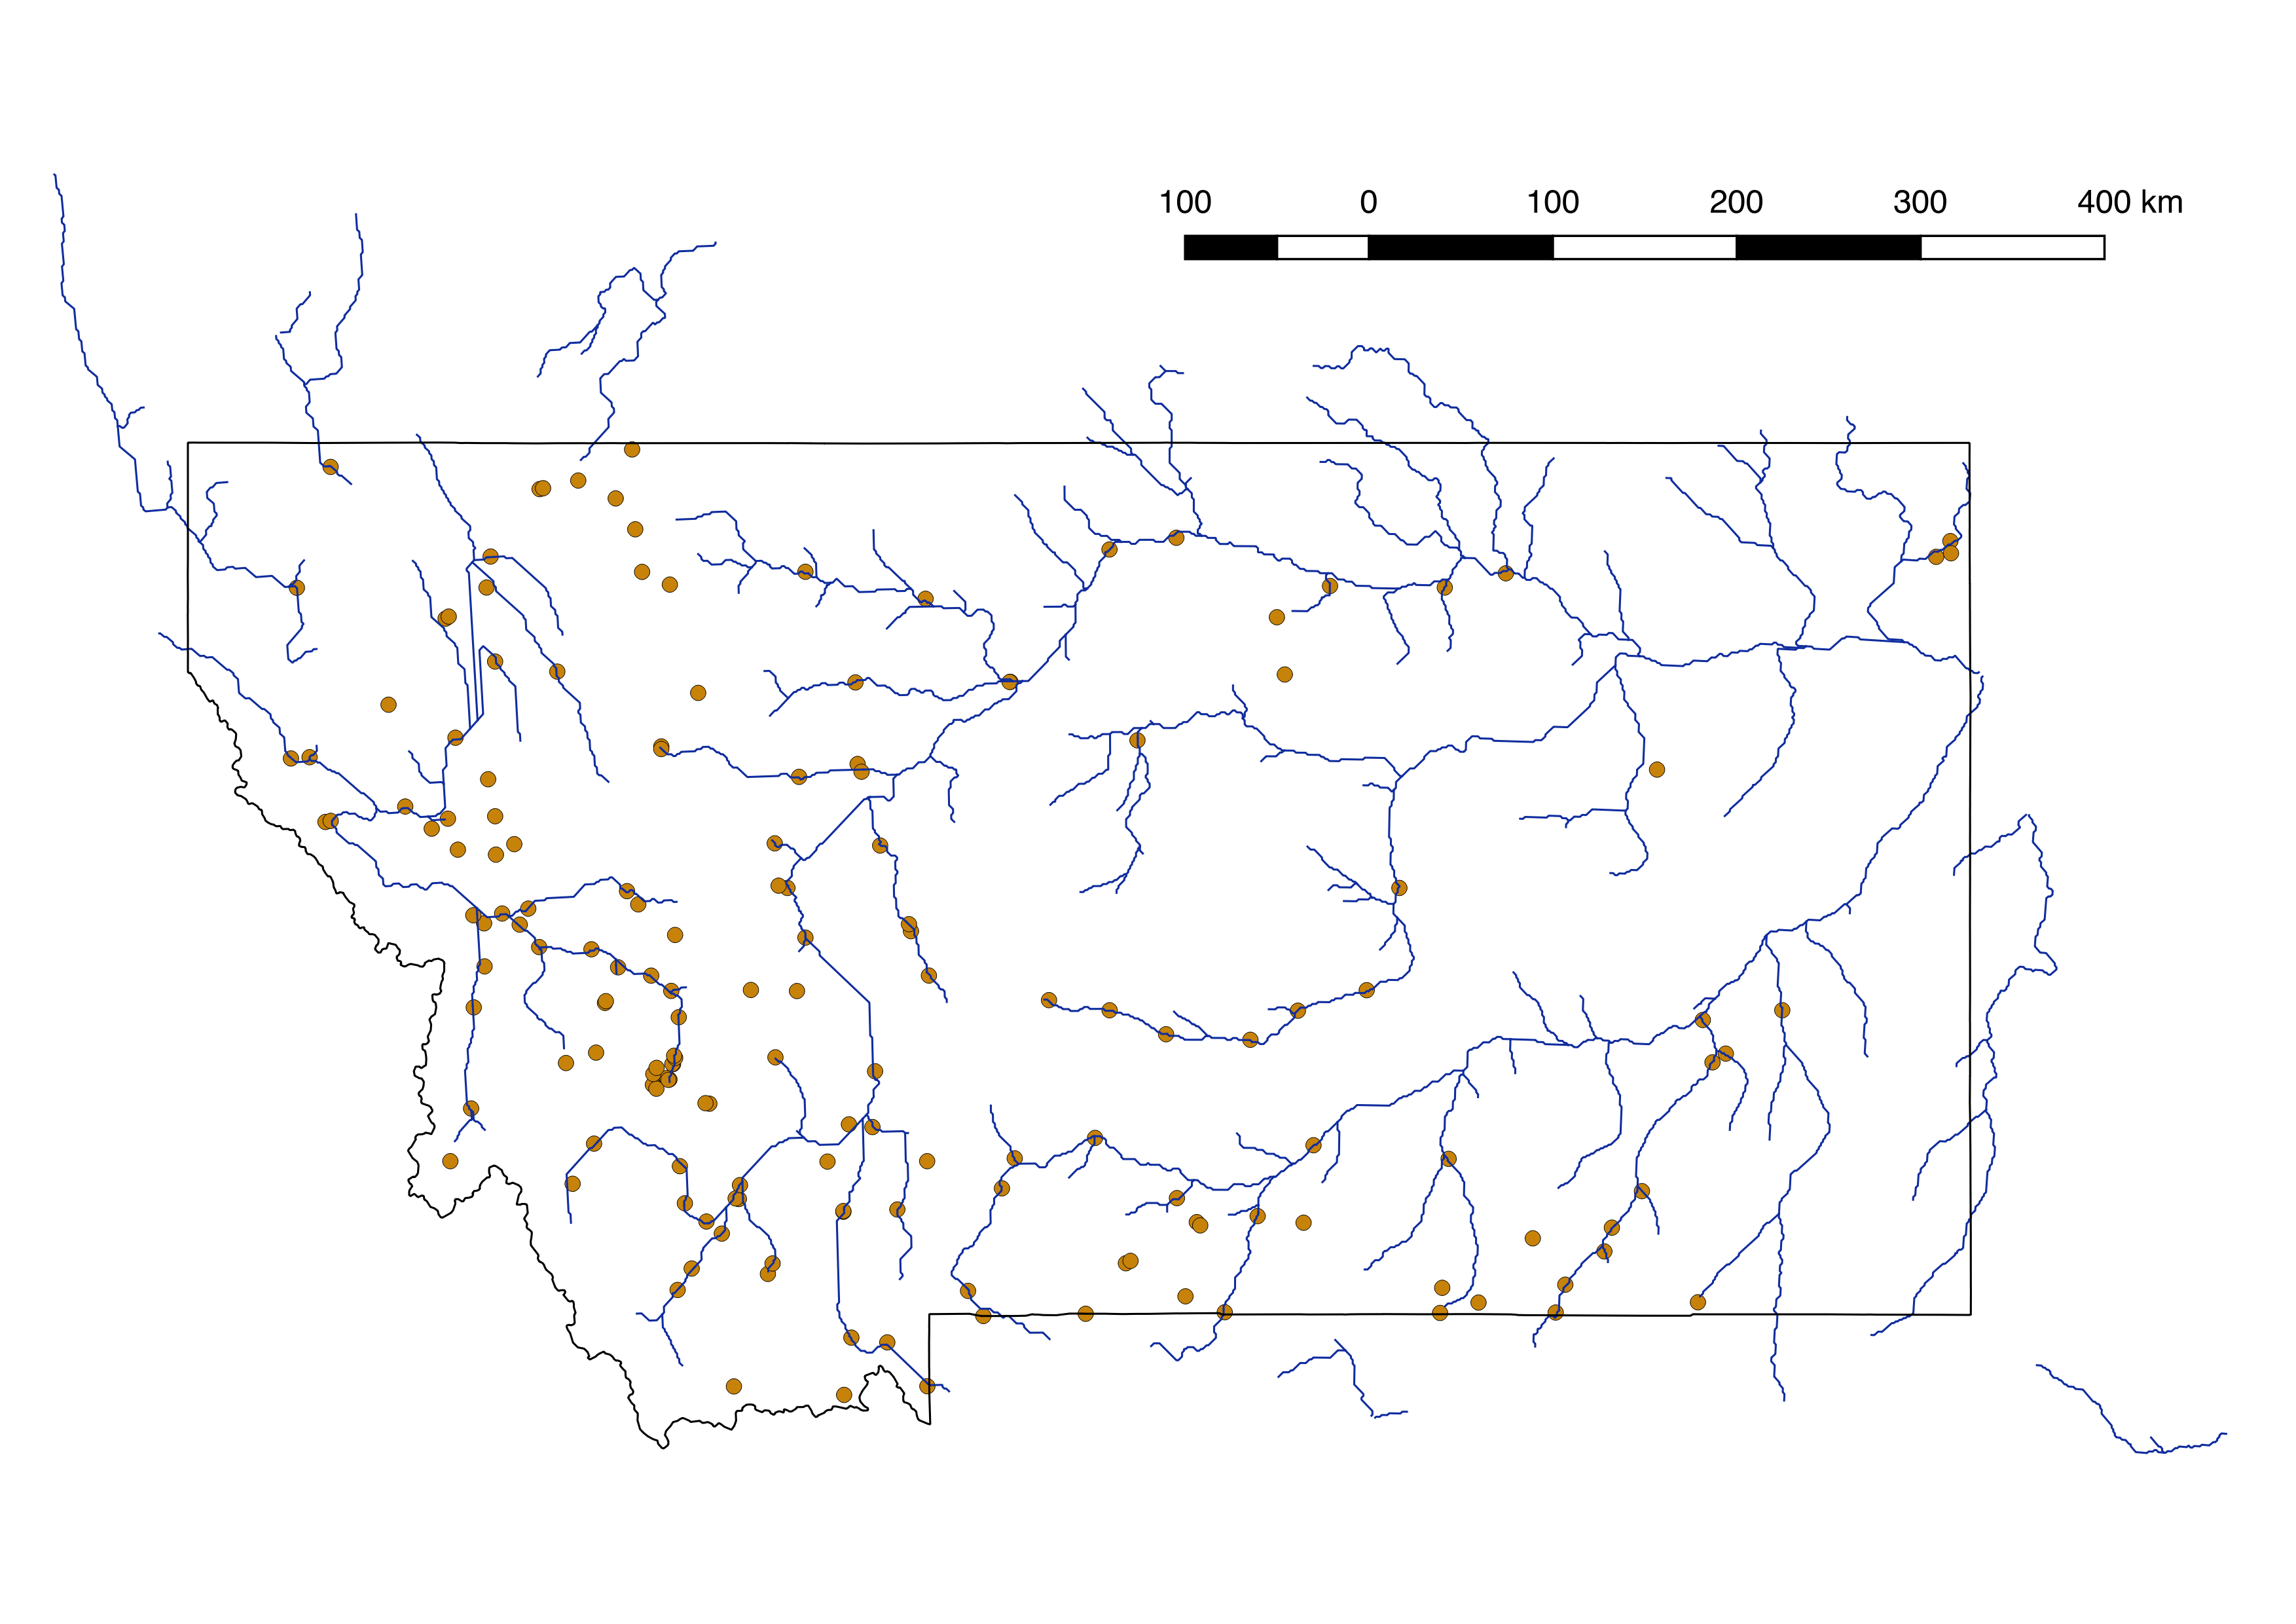
\includegraphics[width=0.95\textwidth]{stations}
    \caption{all SWE stations plotted against modeled streamflows}
    \label{fig:stations}
\end{figure}